\documentclass{beamer}
\usetheme{metropolis}

\usepackage[utf8]{inputenc}
\usepackage[portuguese]{babel}

\usepackage{color}
\usepackage{dirtytalk}
\usepackage{graphicx}
\usepackage{minted}

\title{Minicurso de Java}
\subtitle{Introdução a Java}
\author{João Paulo Taylor Ienczak Zanette}

\begin{document}

\maketitle

\section{O que é programação?}

\section{Introdução a Java}
\subsection{Sobre a linguagem}

\begin{frame}{Princípios}
    \begin{enumerate}
        \item Deve ser "simples, orientada a objetos, e familiar";
        \item Deve ser "robusta e segura";
        \item Deve ser "de arquitetura neutra e portátil";
        \item Deve executar com "alta performance";
        \item Deve ser "interpretada, com threads e dinâmica";
    \end{enumerate}
\end{frame}


\begin{frame}{Características gerais da linguagem}

    \begin{description}
        \item[Multiplataforma:] O mesmo código pode rodar em mais de uma plataforma
            sem a necessidade de recompilar;
        \item[Biblioteca padrão extensa:] Oferece diversos recursos já na
            biblioteca padrão, desde interfaces gráficas até manipulação de
            áudio/vídeo;
        \item[Alocação não-determinística:] Recursos alocados não são liberados
            explicitamente pelo programador, isso é feito por um
            \emph{Garbage-Collector};
        \item[Suporte a JIT:] Alguns trechos de código são otimizados em tempo de
            execução (\textit{Just In Time Compilation}).
    \end{description}

    \say{Java é uma mãezona: não deixa você fazer algo errado e ainda limpa
    tudo para você.}

\end{frame}


\begin{frame}{Onde é utilizada}
    \begin{itemize}
        \item Aplicações Desktop no geral (com ou sem interface gráfica);
        \item Comunicação com Banco de Dados em servidores de aplicações Web
            (\textit{back-end});
        \item Aplicações para dispositivos móveis Android;
        \item Sistemas embarcados e de tempo-real.
    \end{itemize}

    Foi bastante utilizada também para aplicações de celulares antigos (JavaME).
\end{frame}


\begin{frame}{A \textit{Java Virtual Machine}}
    Toda aplicação Java roda na JVM a partir de uma sequência de instruções
    geradas de um código Java. Essas instruções se chamam
    \textbf{\textit{Bytecode}}.
\end{frame}


\begin{frame}{Desenvolvendo uma aplicação Java simples}
    \begin{enumerate}
        \item Crie um arquivo de código Java (.java);
        \item Escreva o código (ver exemplo adiante), definindo o procedimento
            \texttt{main};
        \item Gere o \textit{Bytecode} da aplicação, que será lido pela JVM.
            Isso é feito pelo processo de \emph{Compilação};
        \item Execute o código chamando a JVM e indicando qual classe deve ser
            carregada. A JVM vai procurar e executar o procedimento
            \texttt{main} dessa classe.
    \end{enumerate}
\end{frame}


\begin{frame}[fragile]{Exemplo de código Java}
    \begin{minted}{java}
public class Application {
    public static void main(String... args) {
        System.out.println("Hello, World!");
    }
}
    \end{minted}

    \emph{OBS}: Toda aplicação Java inicia pelo \texttt{main}.
\end{frame}


\begin{frame}{Utilizando o compilador de Java}
    Se estiver utilizando o eclipse, basta executar o comando "Build". Executar
    e aplicação ("Run") também chama o compilador.

    Se estiver em um terminal, basta chamar:

    \texttt{javac Application.java}
\end{frame}


\begin{frame}{Processo de compilação de Java}
    \begin{center}
        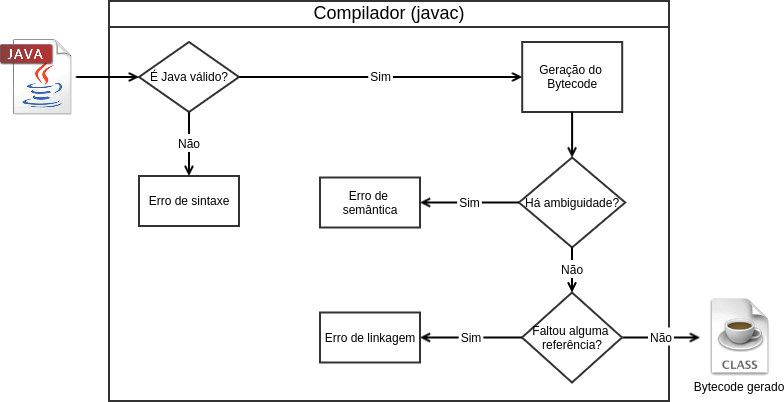
\includegraphics[keepaspectratio,width=1\textwidth,height=1\textheight]{compilation_scheme}
    \end{center}
\end{frame}


\begin{frame}[fragile]{Bytecode gerado}
    \begin{minted}{java}
public class Application {
  public Application();
    Code:
       0: aload_0
       1: invokespecial #1 // java/lang/Object."<init>"
       4: return

  public static void main(java.lang.String...);
    Code:
       0: getstatic     #2 // java/lang/System.out
       3: ldc           #3 // Hello, World!
       5: invokevirtual #4 // java/io/PrintStream.println
       8: return
}
    \end{minted}
\end{frame}


\begin{frame}{Executando uma aplicação Java}
    Se estiver utilizando o Eclipse, basta executar o comando Executar ("Run").

    Se estiver em um terminal, basta chamar:

    \texttt{java Application}
\end{frame}


\begin{frame}{Execução do \textit{Bytecode} Java}
    \begin{center}
        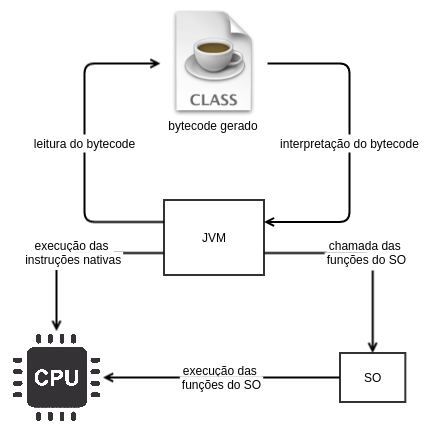
\includegraphics[keepaspectratio,width=1\textwidth,height=0.8\textheight]{jvm_scheme}
    \end{center}
\end{frame}

\end{document}
